\chapter{Código fuente ``\pArm{} \textit{configurator}''}
\label{anex:pArm-configurator}
\lstinputlisting[label={lst:dh_table_py}, style=Python]{pArm-configurator/src/manipulator/dh_table.py}
\lstinputlisting[label={lst:manipulator_py}, style=Python]{pArm-configurator/src/manipulator/manipulator.py}
\section{Enlace a \textit{Jupyter Notebook} para configurar el \pArm}
\label{anex:jupyter_binder}
\url{https://s.javinator9889.com/pArm-config}\qquad
\qrcode{https://s.javinator9889.com/pArm-config}

\chapter{Código fuente S2}
\label{anex:source_code}
\section{\textit{Header files}}
\lstinputlisting[label={lst:planner_h}, style=C]{pArm-S2/pArm.X/arm/planner.h}
\lstinputlisting[label={lst:gcode_h}, style=C]{pArm-S2/pArm.X/gcode/gcode.h}
\lstinputlisting[label={lst:servo_h}, style=C]{pArm-S2/pArm.X/motor/servo.h}
\lstinputlisting[label={lst:motor_h}, style=C]{pArm-S2/pArm.X/motor/motor.h}
\lstinputlisting[label={lst:kinematics_h}, style=C]{pArm-S2/pArm.X/motor/kinematics.h}
\lstinputlisting[label={lst:io_h}, style=C]{pArm-S2/pArm.X/printf/io.h}
\lstinputlisting[label={lst:printf_config_h}, style=C]{pArm-S2/pArm.X/printf/printf_config.h}
\lstinputlisting[label={lst:printf_h}, style=C]{pArm-S2/pArm.X/printf/printf.h}
\lstinputlisting[label={lst:rsa_h}, style=C]{pArm-S2/pArm.X/rsa/rsa.h}
\lstinputlisting[label={lst:rand_h}, style=C]{pArm-S2/pArm.X/rsa/rand.h}
\lstinputlisting[label={lst:zeros_h}, style=C]{pArm-S2/pArm.X/rsa/zeros.h}
\lstinputlisting[label={lst:primes_h}, style=C]{pArm-S2/pArm.X/rsa/primes.h}
\lstinputlisting[label={lst:mutex_h}, style=C]{pArm-S2/pArm.X/sync/mutex.h}
\lstinputlisting[label={lst:barrier_h}, style=C]{pArm-S2/pArm.X/sync/barrier.h}
\lstinputlisting[label={lst:tmr3_h}, style=C]{pArm-S2/pArm.X/timers/tmr3.h}
\lstinputlisting[label={lst:tmr4_h}, style=C]{pArm-S2/pArm.X/timers/tmr4.h}
\lstinputlisting[label={lst:tmr5_h}, style=C]{pArm-S2/pArm.X/timers/tmr5.h}
\lstinputlisting[label={lst:buffer_h}, style=C]{pArm-S2/pArm.X/utils/buffer.h}
\lstinputlisting[label={lst:defs_h}, style=C]{pArm-S2/pArm.X/utils/defs.h}
\lstinputlisting[label={lst:time_h}, style=C]{pArm-S2/pArm.X/utils/time.h}
\lstinputlisting[label={lst:types_h}, style=C]{pArm-S2/pArm.X/utils/types.h}
\lstinputlisting[label={lst:uart_h}, style=C]{pArm-S2/pArm.X/utils/uart.h}
\lstinputlisting[label={lst:utils_h}, style=C]{pArm-S2/pArm.X/utils/utils.h}
\lstinputlisting[label={lst:arm_config_h}, style=C]{pArm-S2/pArm.X/arm_config.h}
\lstinputlisting[label={lst:init_h}, style=C]{pArm-S2/pArm.X/init.h}
\lstinputlisting[label={lst:interrupts_h}, style=C]{pArm-S2/pArm.X/interrupts.h}
\lstinputlisting[label={lst:pragmas_h}, style=C]{pArm-S2/pArm.X/pragmas.h}
\lstinputlisting[label={lst:system_types_h}, style=C]{pArm-S2/pArm.X/system_types.h}


\section{\textit{Source files}}
\lstinputlisting[label={lst:planner_c}, style=C]{pArm-S2/pArm.X/arm/planner.c}
\lstinputlisting[label={lst:gcode_c}, style=C]{pArm-S2/pArm.X/gcode/gcode.c}
\lstinputlisting[label={lst:servo_c}, style=C]{pArm-S2/pArm.X/motor/servo.c}
\lstinputlisting[label={lst:motor_c}, style=C]{pArm-S2/pArm.X/motor/motor.c}
\lstinputlisting[label={lst:kinematics_c}, style=C]{pArm-S2/pArm.X/motor/kinematics.c}
\lstinputlisting[label={lst:printf_c}, style=C]{pArm-S2/pArm.X/printf/printf.c}
\lstinputlisting[label={lst:rsa_c}, style=C]{pArm-S2/pArm.X/rsa/rsa.c}
\lstinputlisting[label={lst:rand_c}, style=C]{pArm-S2/pArm.X/rsa/rand.c}
\lstinputlisting[label={lst:zeros_c}, style=C]{pArm-S2/pArm.X/rsa/zeros.c}
\lstinputlisting[label={lst:primes_c}, style=C]{pArm-S2/pArm.X/rsa/primes.c}
\lstinputlisting[label={lst:mutex_c}, style=C]{pArm-S2/pArm.X/sync/mutex.c}
\lstinputlisting[label={lst:barrier_c}, style=C]{pArm-S2/pArm.X/sync/barrier.c}
\lstinputlisting[label={lst:tmr3_c}, style=C]{pArm-S2/pArm.X/timers/tmr3.c}
\lstinputlisting[label={lst:tmr4_c}, style=C]{pArm-S2/pArm.X/timers/tmr4.c}
\lstinputlisting[label={lst:tmr5_c}, style=C]{pArm-S2/pArm.X/timers/tmr5.c}
\lstinputlisting[label={lst:buffer_c}, style=C]{pArm-S2/pArm.X/utils/buffer.c}
\lstinputlisting[label={lst:time_c}, style=C]{pArm-S2/pArm.X/utils/time.c}
\lstinputlisting[label={lst:uart_c}, style=C]{pArm-S2/pArm.X/utils/uart.c}
\lstinputlisting[label={lst:utils_c}, style=C]{pArm-S2/pArm.X/utils/utils.c}
\lstinputlisting[label={lst:init_c}, style=C]{pArm-S2/pArm.X/init.c}
\lstinputlisting[label={lst:interrupts_c}, style=C]{pArm-S2/pArm.X/interrupts.c}
\lstinputlisting[label={lst:main_c}, style=C]{pArm-S2/pArm.X/main.c}


\newpage
\chapter{Matriz pseudo--inversa cuando $\left|J\left(\dot{q}\right)\right| = 0$}
\label{anex:pinv}
La matriz pseudo--inversa se puede ver desde el siguiente enlace:
\url{https://raw.githubusercontent.com/pArm-TFG/Memoria/master/pictures/equation.svg}\qquad
\qrcode{https://raw.githubusercontent.com/pArm-TFG/Memoria/master/pictures/equation.svg}

\chapter{Código fuente \ac{S1}}
\lstinputlisting[label={lst:connection_py}, style=Python]{pArm-S1/pArm/communications/connection.py}
\lstinputlisting[label={lst:control_py}, style=Python]{pArm-S1/pArm/control/control.py}
\lstinputlisting[label={lst:control_interface_py}, style=Python]{pArm-S1/pArm/control/control_interface.py}
\lstinputlisting[label={lst:control_management.py}, style=Python]{pArm-S1/pArm/control/control_management.py}
\lstinputlisting[label={lst:heart_beat.py}, style=Python]{pArm-S1/pArm/control/heart_beat.py}
\lstinputlisting[label={lst:generator_py}, style=Python]{pArm-S1/pArm/gcode/generator.py}
\lstinputlisting[label={lst:interpreter_py}, style=Python]{pArm-S1/pArm/gcode/interpreter.py}
\lstinputlisting[label={lst:progress_widget_py}, style=Python]{pArm-S1/pArm/GUI/GUI.py}
\lstinputlisting[label={lst:GUI_py}, style=Python]{pArm-S1/pArm/GUI/progress_widget.py}
\lstinputlisting[label={lst:rect_item_py}, style=Python]{pArm-S1/pArm/GUI/rect_item.py}
\lstinputlisting[label={lst:logger_py}, style=Python]{pArm-S1/pArm/logger/logger.py}
\lstinputlisting[label={lst:pyqthandler_py}, style=Python]{pArm-S1/pArm/logger/PyQtHandler.py}
\lstinputlisting[label={lst:rsa_py}, style=Python]{pArm-S1/pArm/security/rsa.py}
\lstinputlisting[label={lst:error_data_py}, style=Python]{pArm-S1/pArm/utils/error_data.py}
\lstinputlisting[label={lst:atomics_py}, style=Python]{pArm-S1/pArm/utils/atomics.py}
\lstinputlisting[label={lst:main_py}, style=Python]{pArm-S1/pArm/__main__.py}
\lstinputlisting[label={lst:app_py}, style=Python]{pArm-S1/app.py}

\begin{landscape}    
    \chapter{Diagrama de Gantt al completo}
    \label{anex:gantt}
    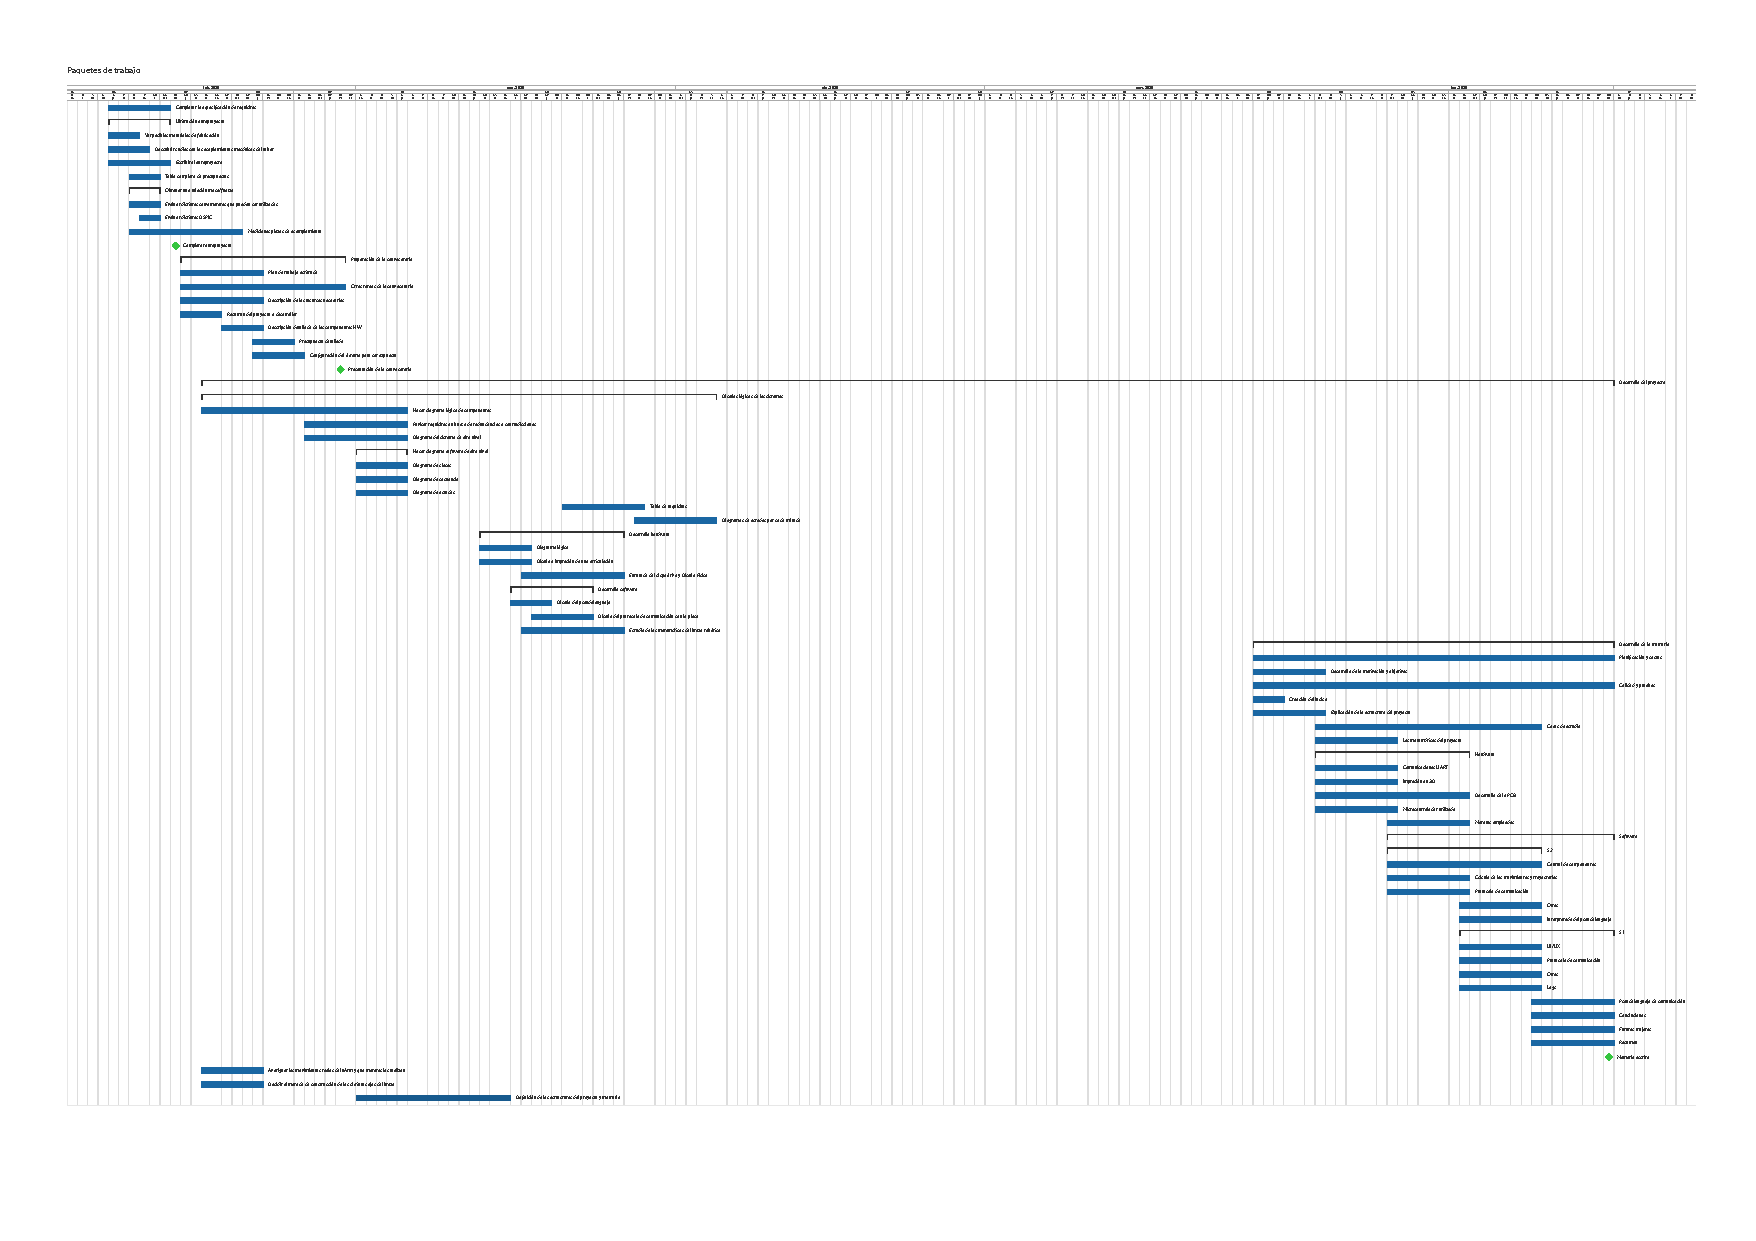
\includepdf[landscape=true]{pictures/gantt_chart.pdf}
\end{landscape}
